\begin{abstract}
%\boldmath
We consider a stochastic  matched subspace detection problem where the signal subspace is unknown and estimated by taking the eigenvalue decomposition of the sample covariance matrix of noisy signal-bearing training data. In moderate to low signal-to-noise ratio (SNR) regimes or in the setting where the number of samples is limited, subspace estimation errors affect the performance of matched subspace detectors. We use random matrix theory to derive an optimal matched subspace detector which accounts for these estimation errors and to analytically predict the associated ROC performance curves. What emerges from the analysis is the importance of using only the $k_\text{eff} \leq k$ \textit{informative} signal subspace components that can be reliably estimated from the noisy, limited data. Specifically, the ROC analysis shows that the performance of the optimal detector matches that of the plug-in detector that uses exactly $k_\text{eff}$ components. The analytical predictions are validated using numerical simulations.
\end{abstract}

\section{Introduction}

\IEEEPARstart{M}{any} signal processing and machine learning problems involve designing a detector to distinguish between signal and noise by using signal-bearing and noise-only training data sets. Subspace-based methods constitute a powerful and widely used class of algorithms for this purpose \cite{hastie2001elements,laaksonen1996subspace,scharf1994matched,jin2005cfar,mcwhorter2003matched}. Matched subspace detectors  solve this problem when the signal-bearing observation can be modeled as residing in a low-dimensional subspace buried in noise. The family of matched subspace detectors developed in \cite{scharf1994matched,jin2005cfar,mcwhorter2003matched} tackle the problem in the setting where the low-dimensional signal subspace is known. Much is known about the performance and optimality properties of these methods. For example, Scharf and Friedlander \cite{scharf1994matched} prove that the generalized likelihood ratio test (GLRT) is optimal for solving matched subspace detection problems while \cite{mcwhorter2003matched} extend this work to the stochastic setting and conclude that the optimal detector in the known noise case is a matched subspace detector.

Much less is known, however, about these detectors in the setting where the signal subspace is unknown and estimated from noisy, limited signal-bearing data. In such settings, when signal-bearing data is available, an estimate of this low-dimensional signal subspace can be formed from an eigen-decomposition of the sample covariance matrix. Standard plug-in detectors form a GLRT test statistic by simply substituting this subspace estimate for the true signal subspace in the expressions found in \cite{mcwhorter2003matched,jin2005cfar} that were derived assuming that the signal subspace was known . However, in the noisy, finite-sample setting, the subspace estimates formed are also noisy. Recent results from random matrix theory (RMT)  precisely quantify these errors in subspace estimation. The primary contribution of this paper is the derivation of a matched subspace detector which explicitly accounts for these predictable subspace estimation errors and the characterization of the receiver operating characteristic (ROC) performance of this detector  relative to the standard plug-in detector.

What emerges from the ROC analysis is the importance of using only the $k_\text{eff} \leq k$ informative signal subspace components that can be reliably estimated from the noisy, limited data as opposed to using the (unknown) intrinsic dimension $k$ of the signal subspace.  Specifically, the ROC analysis shows that the performance of the optimal detector matches that of the plug-in detector that uses exactly $k_\text{eff}$ components. When more than $k_{\text{eff}}$ components are used, the performance of the plug-in detector degrades relative to that of the optimal detector.

The paper is organized as follows. Section \ref{sec:prob} formally states the detection problem. Section \ref{sec:params} highlights pertinent results from random matrix theory that are utilized in Section \ref{sec:detectors} in the derivation of the oracle, plug-in, and optimal matched subspace detectors and in Section \ref{sec:roc} to derive their associated performance metrics. Section \ref{sec:roc} describes a saddlepoint approximation for computing the theoretical ROC curves for the plug-in and optimal detectors. Section \ref{sec:disc} validates our analytical predictions and highlights the importance of picking $k_{\text{eff}}$ over $k$. Concluding remarks are provided in Section \ref{sec:concl}.


\section{Problem Statement}\label{sec:prob}
We consider the detection problem where our observation vector $y \in \mathbb{C}^{n \times 1}$ is modeled as follows:
\begin{equation}\label{eq:prob state}
y=\left\{
\begin{aligned}
&z
&& y\in H_0\\
&Ux+z
&& y\in H_1\\
\end{aligned}\right.
\end{equation}
where $z\sim\mathcal{N}(0,I)$, $U$ is an unknown $n\times k$ (real or complex) matrix with orthonormal columns, and $x\sim\mathcal{N}(0,\Sigma)$ where $\Sigma=\diag(\sigma_1^2,\dots,\sigma_k^2)$ with $\sigma_i^2$ unknown. The dimension of our subspace, $k$, is unknown and $k\ll n$. We also assume that $x$ and $z$ are independent.

To estimate our unknown parameters, $U$ and $\Sigma$, we are given independent signal-bearing training data $\{y_1,\dots,y_m\}$, with $y_i\in H_1 \text{ for } i=1,\dots,m$ and an estimate, $\widehat{k}$ of our unknown dimension, $k$. After forming our subspace estimate, $\widehat{U}$,  we generate our $\widehat{k} \times 1$ test vector $w=\widehat{U}^Hy$. Our goal is to determine a detector, $g(w)\to\{H_0,H_1\}$ which solves the following problem for an unlabeled testing point, $w$:
\begin{equation}\label{eq:maximization}
\begin{aligned}
&\text{maximize}
&& P_D=P\left(g(w)\to H_1 | w\in H_1\right)\\
&\text{subject to}
&& P_F=P\left(g(w)\to H_1 | w\in H_0\right)\leq\alpha\\
\end{aligned}
\end{equation}
where $\alpha\in[0,1]$.

\section{Pertinent Results from RMT}\label{sec:params}
The first step in any detector derivation is to form estimates $\widehat{U}$ and $\widehat{\Sigma}$ to use in a GLRT. We are given signal-bearing training data $\{y_1,\dots,y_m\}$ where $y_i\in H_1$, for $i=1,\dots,m$. which are stacked as columns in a matrix $Y=[y_1,\dots,y_m]$. To form estimates of $U$ and $\Sigma$, we may take the eigenvalue decomposition of the sample covariance matrix, $S=\frac{1}{m}YY^H$. Recent results from random matrix theory allow us to classify the accuracy of eigenvectors and eigenvalues of $S$. From \cite{paul2007asymptotics,asendorf,benaych2011eigenvalues} we have the following result.

\begin{Th}\label{th:angles}
As $n,m \longrightarrow \infty$ with $n/m \to c$ we have that:
\begin{equation*}
\begin{aligned}
&|\langle u_i,\widehat{u}_i\rangle|^2\convas
\begin{cases}
\dfrac{\widehat{\sigma_i}^4-c}{\widehat{\sigma}_{i}^4+\widehat{\sigma}_{i}^2c} & \text{ if } \sigma_{i}^2>\sqrt{c}\\
0 & \textrm{otherwise}\\
\end{cases}\\
&\langle u_i,\widehat{u}_j\rangle ^2\convas 0 \qquad \textrm{ for } i \neq j\\
\end{aligned},
\end{equation*}
where $\widehat{u}_i$ is the $i^{\text{th}}$ eigenvector of $S$.
\end{Th}

Note that the proof of the case where $i\neq j$ will appear in a later journal publication \cite{asendorf}. The key point of Theorem \ref{th:angles} is that only the eigenvectors corresponding to eigenvalues above the phase transition $\sqrt{c}$ are \textit{informative}. When a signal eigenvalue drops below that critical threshold, the corresponding eigenvector estimate is essentially noise-like  (i.e. $|\langle u_i,\widehat{u}_i\rangle|^2=o_{p}(1)$) and thus \textit{uninformative}. The term $|\langle u_i,\widehat{u}_i\rangle|^2$ quantifies mismatch between the estimated and underlying eigenvectors and plays an important role in the performance analysis of the resulting detectors; a similar term also comes up in the analysis of the resolving power of arrays due to model mismatch such as in \cite{cox1973resolving}. Following \cite{nadakuditi2008sample}, we define the effective number of identifiable subspace components $k_\text{eff}$ as:
\begin{equation}\label{eq:keff}
\boxed{k_\text{eff} = \text{Number of } \sigma_i^2\geq\sqrt{c}}
\end{equation}
Intuitively we expect a degradation in the performance of detectors  that utilize subspace components for which $|\langle u_i,\widehat{u}_i\rangle|^2=o_{p}(1)$.  We now turn to the signal eigenvalue estimation problem. Since we are only interested in the signal eigenvalues above the critical value, we apply theorem 3 of \cite{paul2007asymptotics} to our problem.

\begin{Th}\label{th:eigenvalues}
As $n,m \longrightarrow \infty$ with $n/m \to c$, when $\sigma_i^2 > \sqrt{c}$, we have that:
\begin{equation*}
\widehat{\sigma}_i^2\sim f_{\widehat{\sigma}_i^2}(\sigma_i) := \mathcal{N}\left(\left(c+\sigma_i^2+\frac{c}{\sigma_i^2}\right),\frac{2\left(\sigma_i^2+1\right)^2}{\beta n}\left(1-\frac{c}{\sigma_i^4}\right)\right),
\end{equation*}
where $\beta = 1$ when the data is real-valued and $\beta = 2$ when the data is complex-valued.
\end{Th}

We form an estimate of the signal eigenvalue, $\sigma_{i}^{2}$, by employing maximum-likelihood (ML) estimation on $\widehat{\sigma}_i$. Specifically, we form the estimate:
\begin{equation}\label{eq:cov}
\widehat{\sigma}^2_{i_\text{rmt}} = \argmax_{\sigma_i^2} \log\left(f_{\widehat{\sigma}_i^2}(\sigma_i)\right)
\end{equation}
for only the $k_\text{eff}$ signal eigenvalues for which $\sigma_i^2 > \sqrt{c}$.  We estimate $k_\text{eff}$ by (say) using ``Algorithm 2'' of  \cite{nadakuditi2010fundamental}.  Knowing $\widehat{\sigma}^2_{i_\text{rmt}}$ from data, we can now estimate $|\langle u_i,\widehat{u}_i\rangle|^2$ by an application of Theorem \ref{th:angles}. We refer to this estimate as $|\langle u_i,\widehat{u}_i\rangle|^2_{\text{rmt}}$.

\section{Family of Matched Subspace Detectors}\label{sec:detectors}

The Neyman-Pearson Lemma (see \cite{van1968detection}) states that the solution to (\ref{eq:maximization}) is a likelihood ratio test (LRT)
\begin{equation*}
\Lambda(w) \detgtrless \eta
\end{equation*}
where $\Lambda(w) = \frac{f(w|H_1)}{f(w|H_0)}$ and $\eta$ satisfies $P(\Lambda(w)\leq\eta|H_0)=\alpha$. The LRT relies on the conditional distributions of our test statistic under each hypothesis, which by properties of Gaussian random variables are simply
\begin{equation*}
\begin{aligned}
&w|H_0\sim\mathcal{N}(0,I_{\widehat{k}})\\
&w|H_1\sim\mathcal{N}(0, \widehat{U}^HU\Sigma U^H\widehat{U} +I_{\widehat{k}})\\
\end{aligned}
\end{equation*}

\subsection{Detectors Considered}\label{sec:main results}

We will consider three different detectors for our test data $w$. The first is an oracle detector, which will assume that $U$ and $\Sigma$ are known. The purpose of this is to give an upper bound on a detector's performance. The second is a plug-in detector which uses the oracle statistic and plugs in our estimates of $\widehat{U}$  and $\widehat{\Sigma}$ for our unknown $U$ and $\Sigma$ with the additional assumption that $\widehat{U} = U$ and $\widehat{\Sigma} = \Sigma$. The third is the optimal, new detector which explicitly exploits the quantification of the subspace accuracy estimates in Theorem \ref{th:angles} and only $\widehat{k} = k_\text{eff}$ subspace components to form an approximation to the oracle classifier . Table \ref{table: main results} summarizes the test statistic derived for each detector and the distribution under each hypothesis.

\begin{table*}[!ht]
\centering
\begin{tabular}{cclclcl}\toprule
 Detector & \phantom{a} & Detector Statistic $\Lambda(w)$ & \phantom{a} & Null Hypothesis Distribution $\Lambda|H_0$& \phantom{a} & Simple Hypothesis Distribution $\Lambda|H_1$\\
\midrule
Oracle && $ w^H\left[I-\left(\widehat{U}^HU\Sigma U^H\widehat{U}+I\right)^{-1}\right]w$ &&  && \\
Plug-in && $\sum_{i=1}^{\widehat{k}}w_i^2\frac{\widehat{\sigma}_i^2}{1+\widehat{\sigma}_i^2}$ && $\sum_{i=1}^{\widehat{k}}\left(\frac{\widehat{\sigma}_i^2}{1+\widehat{\sigma}_i^2}\right)\chi^2_{1i}$ && $\sum_{i=1}^{\widehat{k}}\left(\frac{\widehat{\sigma}_i^2\left(1+\sigma^2_i|\langle u_i,\widehat{u}_i\rangle|^2\right)}{1+\widehat{\sigma}_i^2}\right)\chi^2_{1i}$\\
%Energy &&$\sum_{i=1}^{\widehat{k}} w_i^2 $ && $\chi^2_{{\widehat{k}}}$ && $\sum_{i=1}^{\widehat{k}}\left(\sigma^2_i|\langle u_i,\widehat{u}_i\rangle|^2+1\right)\chi^2_{1i}$\\
 Optimal&& $\sum_{i=1}^{\min\{k_\text{eff},\widehat{k}\}}w_i^2\frac{|\langle u_i,\widehat{u}_i\rangle|^2_{\text{rmt}}\widehat{\sigma}_{i_\text{rmt}}^2}{1+|\langle u_i,\widehat{u}_i\rangle|^2_{\text{rmt}}\widehat{\sigma}_{i_\text{rmt}}^2 }$ && $\sum_{i=1}^{\min\{k_\text{eff},\widehat{k}\}}\left(\frac{\widehat{\sigma}_{i_\text{rmt}}^2|\langle u_i,\widehat{u}_i\rangle|^2_{\text{rmt}}}{1+\widehat{\sigma}_{i_\text{rmt}}^2|\langle u_i,\widehat{u}_i\rangle|^2_{\text{rmt}}}\right)\chi^2_{1i}$ && $\sum_{i=1}^{\min\{k_\text{eff},\widehat{k}\}}\left(\widehat{\sigma}^2_{i_\text{rmt}}|\langle u_i,\widehat{u}_i\rangle|^2_{\text{rmt}}\right)\chi^2_{1i}$\\
\bottomrule
\end{tabular}
\caption{Given an observation vector $y$ we form the vector $w=\widehat{U}^Hy$ where $\widehat{U}$ is an estimate of the signal subspace. The table summarizes the test statistic associated with each detector and the associated distribution under $H_0$ and $H_1$. In the CFAR setting, the threshold is  set to obtain the desired false alarm probability. Note the appearance of $k_\text{eff}$ in the optimal detector.}\vskip-0.2cm
\label{table: main results}
\end{table*}

\subsection{Oracle Detector}\label{sec:oracle}

The oracle detector assumes that $\Sigma$ and $U$ are both known. The LRT statistic for our processed data $w$ is
\begin{equation*}
\Lambda(w)=\frac{\mathcal{N}(0,\widehat{U}^HU\Sigma U^H\widehat{U} +I)}{\mathcal{N}(0,I_{\widehat{k}})}
\end{equation*}
After simplification of this expression using the natural logarithm operator as a monotonic operation, the oracle statistic becomes
\begin{equation}\label{eq:oracle stat}
\boxed{\Lambda_{\text{oracle}}(w) = w^H\left[I-\left(\widehat{U}^HU\Sigma U^H\widehat{U}+I\right)^{-1}\right]w}
\end{equation}
and the oracle detector is
\begin{equation}\label{eq:oracle classifier}
\boxed{\Lambda_{\text{oracle}}(w) \detgtrless \ln(\eta_{\text{oracle}})}
\end{equation}
where $\eta_{\text{oracle}}$ satisfies $P(\Lambda_{\text{oracle}}(w)\leq\ln\left(\eta_{\text{oracle}}\right)|H_0)=\alpha$.

\subsection{Plug-in Detector}\label{sec:plugin}

As is the case in this particular problem, $U$ and $\Sigma$ are unknown, and therefore (\ref{eq:oracle stat}) cannot be computed directly. One may then substitute ML estimates for the unknown parameters in the oracle detector to form a GLRT as in \cite{jin2005cfar} and \cite{mcwhorter2003matched}. The ML estimates (in the large-sample, small matrix setting) for $U$ and $\Sigma$ are:
\begin{equation}\label{eq:param estims}
\begin{aligned}
&\widehat{U}=[\widehat{u}_1 \dots \widehat{u}_{\widehat{k}}]\\
&\widehat{\sigma}_i^2 = \lambda_i -1 \text{ for } i=1,\dots,\widehat{k}\\
\end{aligned}
\end{equation}
where $\lambda_1,\dots,\lambda_{\widehat{k}}$ are the largest $\widehat{k}$ eigenvalues of $S$ and $\widehat{u}_1,\dots,\widehat{u}_{\widehat{k}}$ are the corresponding eigenvectors. Define the signal covariance matrix estimate as $\widehat{\Sigma}=\diag(\widehat{\sigma}_1^2,\dots,\widehat{\sigma}_{\widehat{k}}^2)$.

By replacing the unknown parameters in (\ref{eq:oracle stat}) with the estimated parameters in (\ref{eq:param estims}), the plug-in detector statistic becomes:
\begin{equation*}
\Lambda_{\text{plugin}}(w)= w^H\left(I-\left[\widehat{U}^H\widehat{U}\widehat{\Sigma}\widehat{U}^H\widehat{U} + I\right]^{-1}\right)w\\
\end{equation*}
This simplifies to
\begin{equation}\label{eq:plugin stat}
\boxed{\Lambda_{\text{plugin}}(w) = w^H\diag\left(\frac{\widehat{\sigma}^2_i}{1+\widehat{\sigma}^2_i}\right)w=\sum_{i=1}^{\widehat{k}}w_i^2\frac{\widehat{\sigma}_i^2}{\widehat{\sigma}_i^2+1}}
\end{equation}
and our detector becomes
\begin{equation}\label{eq:plugin classifier}
\boxed{\Lambda_{\text{plugin}}(w) \detgtrless \ln(\eta_{\text{plugin}})}
\end{equation}
where $\eta_{\text{plugin}}$ satisfies $P(\Lambda_{\text{plugin}}(w)\leq\ln\left(\eta_{\text{plugin}}\right)|H_0)=\alpha$.

The plug-in detector assumes that the estimated signal subspace $\widehat{U}$ is equal to the true signal subspace $U$ and that the estimated signal covariance $\widehat{\Sigma}$ is equal to the true signal covariance $\Sigma$. It also assumes that the provided subspace dimension estimate $\widehat{k}$ is equal to the true underlying dimension of our signal subspace $k$. However, as shown in Section \ref{sec:params}, choosing $\widehat{k} > k_\text{eff}$ leads to a degradation in the performance of the plug-in detector.

\subsection{Optimal Detector}\label{sec:optimal}

Consider the covariance matrix of the conditional distribution $w|H_1$. By Theorem \ref{th:angles} and additional analysis omitted here for brevity (see \cite{asendorf}), we have that in the large matrix limit:
\begin{equation}\label{eq:cov mat}
\widehat{U}^HU\Sigma U^H\widehat{U}+I = \diag\left(|\langle u_i,\widehat{u}_i\rangle|^2\sigma_i^2 + 1 + o_{p}(1)\right).
\end{equation}
The plug-in detector assumes that $|\langle u_i,\widehat{u}_i\rangle|^2=1$ and $\widehat{\sigma}_i^2=\sigma_i^2$. Theorems \ref{th:angles} and \ref{th:eigenvalues} show that this assumption is invalid because these eigenvalue and eigenvector estimates are biased. Although, $\sigma_i^2$ and $|\langle u_i,\widehat{u}_i\rangle|^2$ are unknown, we already derived an improved signal variance estimate in (\ref{eq:cov}). We plug this estimate into Theorem \ref{th:angles} to obtain an estimate for $|\langle u_i,\widehat{u}_i\rangle|^2$, which we denote $|\langle u_i,\widehat{u}_i\rangle|^2_\text{rmt}$. We then derive an optimal detector by substituting these random matrix theory estimates into the diagonal covariance matrix (\ref{eq:cov mat}) and using this covariance matrix in the GLRT. This choice is well-motivated in the high-dimensional setting where we can ignore the $o_{p}(1)$ terms on the right hand side of (\ref{eq:cov mat}). After simplification of the GLRT, the optimal statistic is
\begin{equation*}
\Lambda_{\text{optimal}}(w)= \sum_{i=1}^{\widehat{k}}w_i^2\frac{|\langle u_i,\widehat{u}_i\rangle|^2_{\text{rmt}}\widehat{\sigma}_{i_\text{rmt}}^2}{|\langle u_i,\widehat{u}_i\rangle|^2_{\text{rmt}}\widehat{\sigma}_{i_\text{rmt}}^2 + 1}
\end{equation*}
However, as $|\langle u_i,\widehat{u}_i\rangle|^2=0$ when $\widehat{\sigma}_{i_\text{rmt}}^2$ drops below $\sqrt{c}$, this sum ignores all indices whose signal eigenvalue estimate is below this critical value. Instead, the optimal detector only sums those components with significant signal eigenvalues. The number of significant signal eigenvalues was defined as $k_\text{eff}$. Our final optimal statistic  thus becomes:
\begin{equation}\label{eq:rmt stat}
\boxed{\Lambda_{\text{optimal}}(w)= \sum_{i=1}^{\min\{k_\text{eff},\widehat{k}\}}w_i^2\frac{|\langle u_i,\widehat{u}_i\rangle|^2_{\text{rmt}}\widehat{\sigma}_{i_\text{rmt}}^2}{|\langle u_i,\widehat{u}_i\rangle|^2_{\text{rmt}}\widehat{\sigma}_{i_\text{rmt}}^2 + 1}}
\end{equation}
and the optimal detector becomes
\begin{equation}\label{eq:rmt classifier}
\boxed{\Lambda_{\text{optimal}}(w) \detgtrless \ln(\eta_{\text{optimal}})}
\end{equation}
where $\eta_{\text{optimal}}$ satisfies $P(\Lambda_{\text{optimal}}(w)\leq\eta_{\text{optimal}}|H_0)=\alpha$.

\section{Theoretical ROC Curve Derivation}\label{sec:roc}
A standard way to compare the plug-in and optimal detectors derived in (\ref{eq:plugin classifier}) and (\ref{eq:rmt classifier}) respectively is to compute their ROC curves \cite{fawcett2006introduction}. For a particular statistic $\Lambda(w)$, to compute theoretical ROC curves, we must compute
\begin{equation}\label{eq:target cdf}
\begin{aligned}
&P_D = P(\Lambda(w) \geq y| w\in H_1)\\
&P_F = P(\Lambda(w) \geq y| w\in H_0)\\
\end{aligned}
\end{equation}
for $-\infty<y<\infty$. To do this, we explore the conditional CDF under each hypothesis for the statistics (\ref{eq:plugin stat}) and (\ref{eq:rmt stat}).

The conditional distributions of our test samples under each hypothesis are $w|H_0\sim\mathcal{N}(0,I)$ and $w|H_1\sim\mathcal{N}(0,\widehat{U}^HU\Sigma U^H\widehat{U}+I)$. Because of the diagonal covariance matrix under $H_0$, $w_i|H_0\sim\mathcal{N}(0,1)$ are i.i.d for $i=1,\dots,\widehat{k}$ and $w_i^2|H_0\sim\chi_1^2$ are i.i.d for $i=1,\dots,\widehat{k}$. As argued in (\ref{eq:cov mat}), the covariance matrix under $H_1$ is asymptotically diagonal. We have that $w_i|H_1\approx\mathcal{N}(0,\sigma^2_i|\langle u_i,\widehat{u}_i\rangle|^2+1)$ are i.i.d for $i=1,\dots,\widehat{k}$. Therefore, for $i=1,\dots,\widehat{k}$
\begin{equation*}
\frac{w_i^2|H_1}{\sigma^2_i|\langle u_i,\widehat{u}_i\rangle|^2+1}\sim\chi_1^2
\end{equation*}
The third and fourth columns of Table \ref{table: main results} summarize the sample conditional distributions for $w$ into each detector's statistic.  An analytical expression for the asymptotic performance in the large matrix limit  is obtained by substituting expressions from Theorems \ref{th:angles} \& \ref{th:eigenvalues} for the pertinent quantities in these distributions. Note that all distributions are a weighted sum of independent chi-square random variables with one degree of freedom. That is the distributions take the form
\begin{equation*}
\Lambda = \sum_{i=1}^r\beta_i\chi^2_{1i}
\end{equation*}
where $\beta_i$ is the appropriate weighting, unique to each statistic under each hypothesis. The CDF of a chi-square random variable is known in closed form. However, the CDF of a weighted sum of independent chi-square random variables is not known in closed form. To evaluate (\ref{eq:target cdf}), we use a saddlepoint approximation of the CDF of $\Lambda$ by employing the generalized Lugannani-Rice formula proposed in \cite{wood1993saddlepoint}. To then compute a theoretical ROC curve, $y$ is swept over $(0,\infty)$ and for each value of $y$, the saddlepoint approximation of the CDF under each hypothesis is computed using the method alluded to. This generates a set of points $(P_F,P_D)$ which approximate the theoretical ROC curve. Figure \ref{fig:roc} illustrates the result of one such computation.

\begin{figure}
\centering
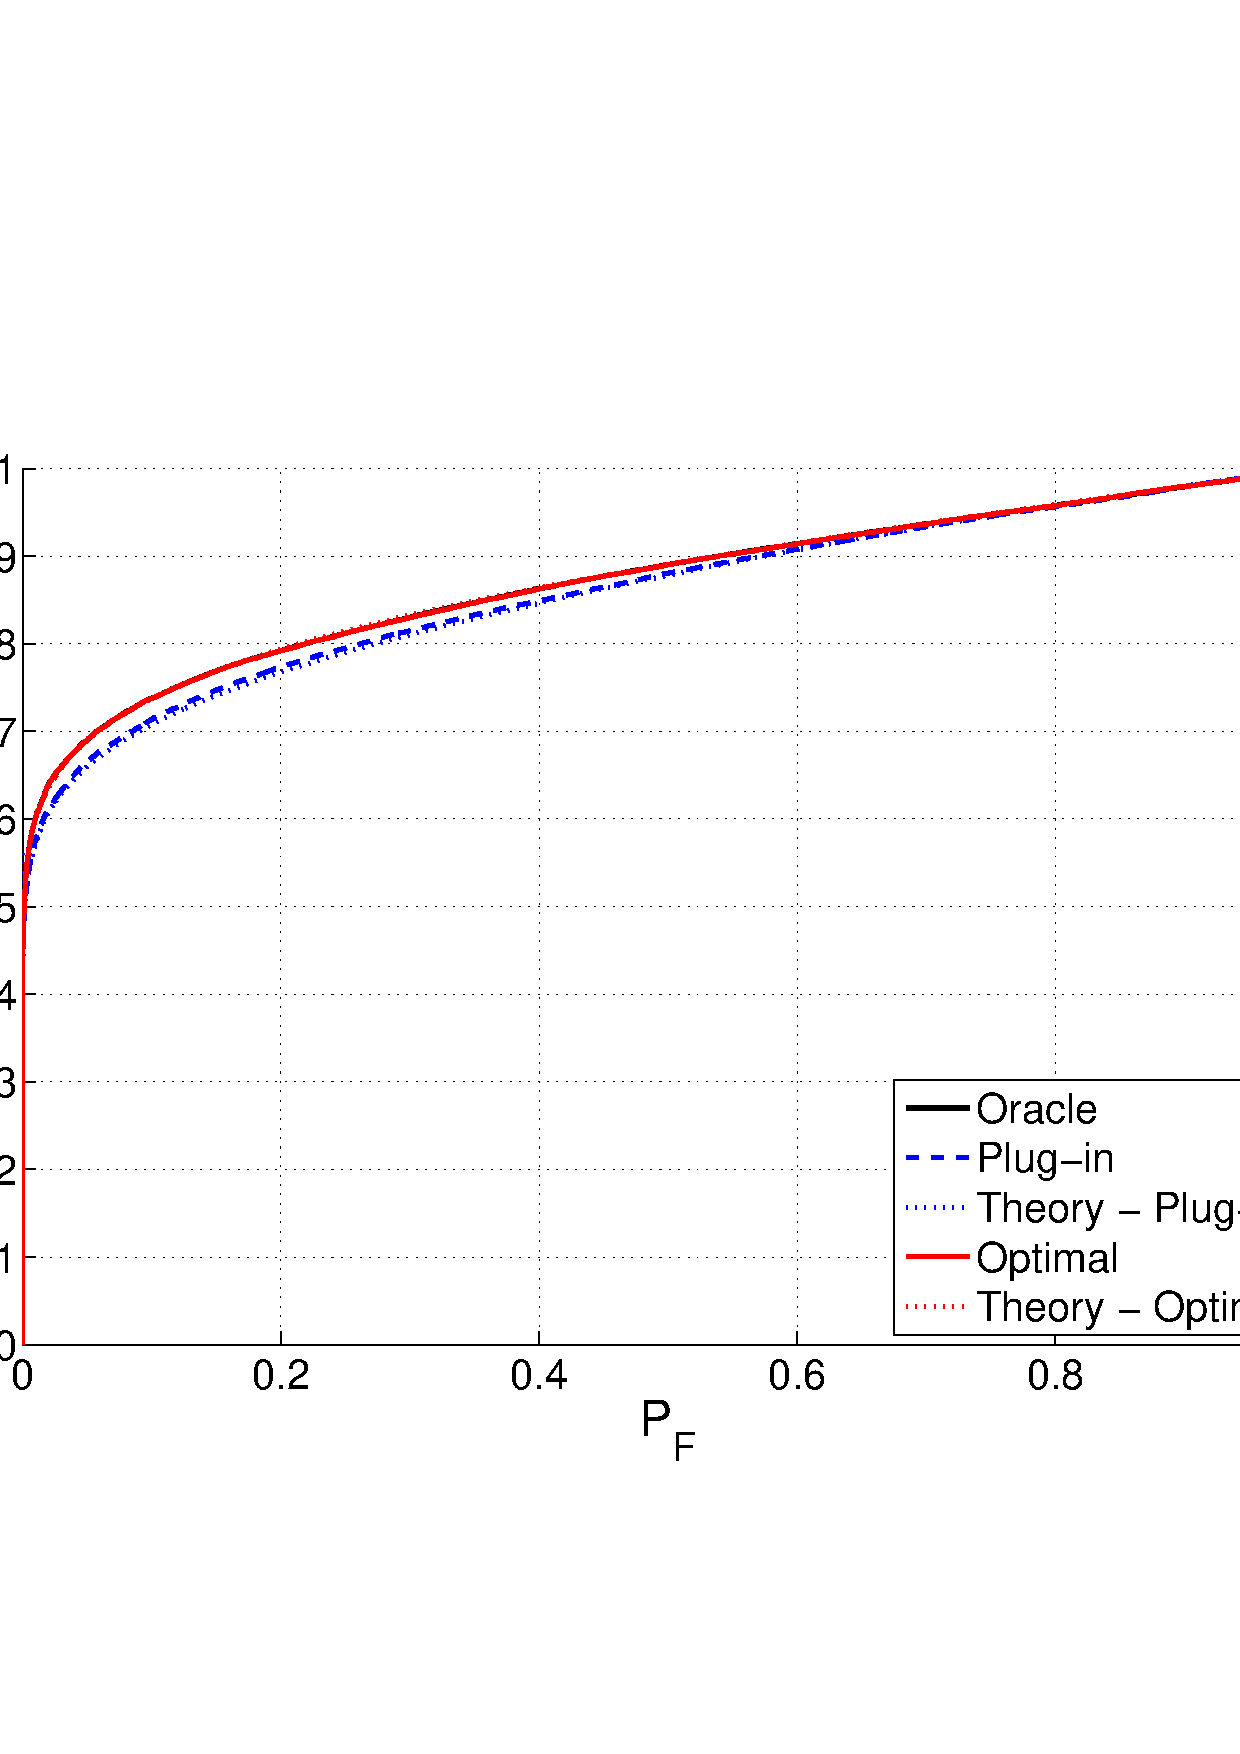
\includegraphics[width=3.5in]{figures/roc_curves.png}
\caption{Empirical and theoretical ROC curves for the oracle, plug-in, and optimal matched subspace detectors. Empirical ROC curves were simulated with $n=100$, $m=50$, $k=2$, $\widehat{k}=2$, $\sigma_1=5$, $\sigma_2=0.5$. However, as $\sigma_2$ is below the critical threshold, $k_{\text{eff}} = 1$. The empirical ROC curves were computed using $2000$ test samples and averaged over 25 trials using algorithms 2 and 4 of \cite{fawcett2006introduction}. The theoretical ROC curves were computed as described in Section \ref{sec:roc}. Since we chose $\widehat{k} > k_{\text{eff}}$, we observe a performance gain when using the optimal detector. In fact, the optimal detector operates at almost the same $(P_F, P_D)$ as the oracle detector. The theoretically predicted ROC curves match the empirical results reflecting the accuracy of the approximations employed. }\vskip-0.15cm
\label{fig:roc}
\end{figure}

\begin{figure}
\centering
\includegraphics[width=3.5in]{figures/k_hat_graph.png}
\caption{Empirical exploration of the achieved probability of detection, $P_D$, for a fixed probability of false alarm, $P_F=0.01$, for various $\widehat{k}$. For the simulation, $n=100$, $m=50$, $k=6$, $\Sigma^{1/2} = \diag({\bf{5,4,3,2}},0.6,0.5)$ so that $k_{\text{eff}}=4$. $P_D$ calculation was computed using 2000 test samples and averaged over 25 trials. The optimal $\widehat{k}$ resulting in the largest $P_D$ is not the true $k$, but rather $k_\text{eff}$.}\vskip-0.15cm
\label{fig:khat}
\end{figure}


\section{Simulation Results and Discussion}\label{sec:disc}

\subsection{ROC curves}
As seen in Figure \ref{fig:roc}, the theoretical ROC curves match the empirical ROC curves thereby validating the accuracy of the saddlepoint approximation to the CDF. The performance of the optimal detector matches that of the oracle detector attesting to the accuracy of the random matrix theoretic approximations employed. Finally, we note the sub-optimality of the plug-in detector. This is expected as we chose $\widehat{k} > k_\text{eff}$ so that the additional subspace component chosen was uninformative.

\subsection{Optimality of $k_\text{eff}$}
Figure \ref{fig:khat} examines the performance as a function of $\widehat{k}$, confirming our assertion that the optimal $\widehat{k}$ equals $k_\text{eff}$. Setting $\widehat{k} < k_\text{eff}$ drastically degrades performance for both detectors. Notably, the plug-in and optimal detectors realize the same ROC performance demonstrating that quantification and exploitation of the subspace estimation accuracy, while useful in ROC performance prediction, does \textit{not} noticeably enhance detection performance. When $\widehat{k} > k_\text{eff}$, the performance of the plug-in detector degrades while that of the optimal detector is relatively stable as if $\widehat{k}=k_\text{eff}$. In other words, we do not pay a price for overestimating our dimension with the optimal detector.

This makes sense (and is slightly contrived) because the optimal detector will only sum to a maximum of $k_\text{eff}$ indices as evident in (\ref{eq:rmt stat}). In many applications, practitioners might employ the ``play-it-safe'' approach and set $\widehat{k}$ to be slightly greater than $k_\text{eff}$. The degradation in performance by adding each uninformative subspace, as seen in Figure \ref{fig:khat}, constitutes evidence to our assertion that overestimating the signal subspace dimension is a bad idea. The plug-in detector achieves optimal performance whenever $\widehat{k} = k_\text{eff}$. When $k_\text{eff} < k$, setting $\widehat{k} = k$ is sub-optimal.

\subsection{Averaging over Test Samples}
Figure \ref{fig:samples} shows the performance in the setting where the test statistic is averaged over multiple independent samples. Here $k_\text{eff} = 2$ and the plug-in estimator sets $\widehat{k} = 6$. The optimal detector requires less samples than the plug-in detector to achieve a desired $(P_F, P_D)$ pair. This arises from the fact that the optimal detector discards the uninformative signal subspace components while the plug-in detector utilizes them. Because each test sample is pruned to ignore noisy components, we can average less samples to achieve a desired accuracy.

\section{Conclusion}\label{sec:concl}
We have considered a stochastic  matched subspace detection problem where the signal subspace is unknown and estimated from noisy, limited signal-bearing training data. We used random matrix theory to analytically characterize the ROC performance of a family of matched subspace detectors including a new, optimal detector that exploits information about the ``noisiness'' of the signal subspace estimates.

What emerges from the analysis is the fact that quantification of whether an estimated subspace is informative or not, is more important than the relative degree of noisiness. The effective number of identifiable subspace components $k_\text{eff}$, first introduced in \cite{nadakuditi2008sample}, and expressed in (\ref{eq:keff}), affects detector performance the most. When $\widehat{k} = k_\text{eff}$, the standard plug-in detector is near-optimal; when $\widehat{k} \neq k_\text{eff}$, it is not. This highlights the importance of robust techniques \cite{johnstone2001distribution,el2007tracy,nadakuditi2010fundamental} for estimating $k_\text{eff}$ in subspace based detection schemes. We are working on extending the analysis to deterministic matched subspace detectors.

\begin{figure}
\centering
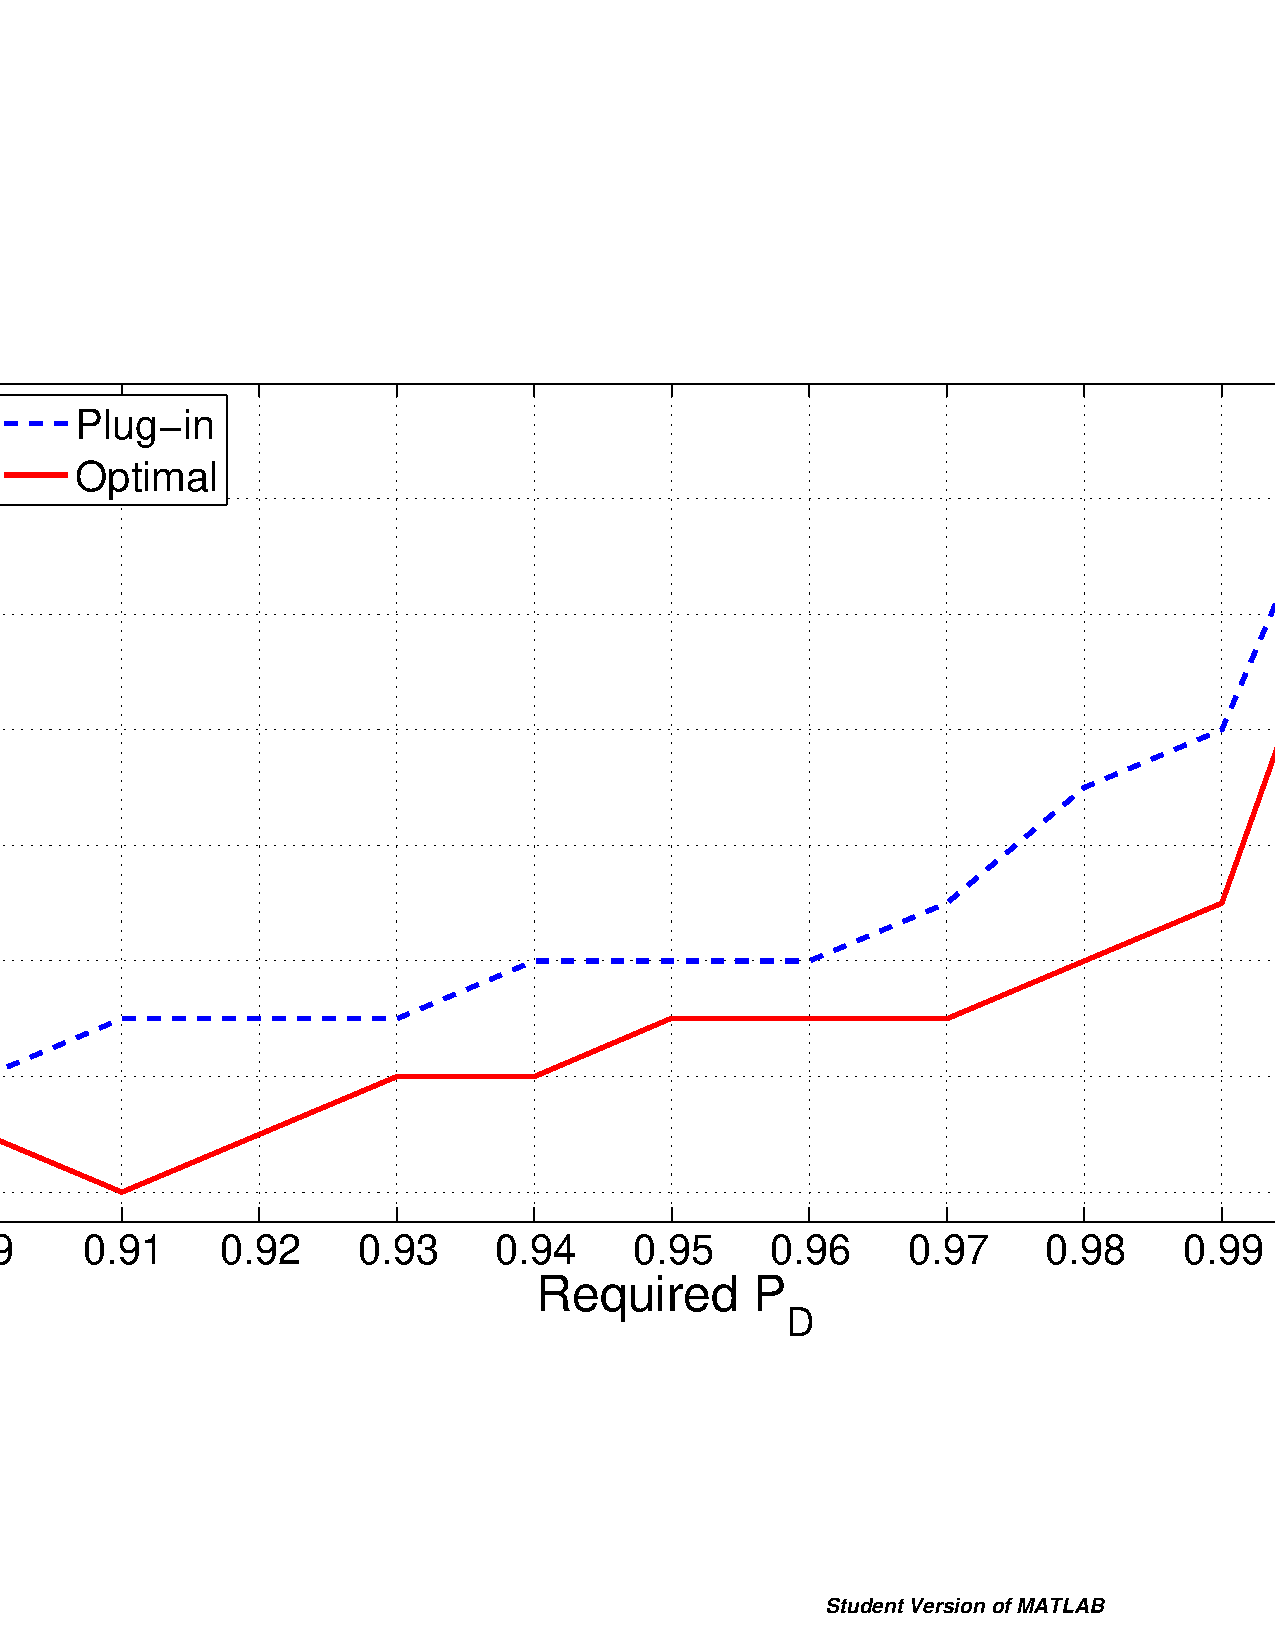
\includegraphics[width=3.5in]{figures/samples_graph.png}
\caption{Empirical exploration of the number of test samples required to achieve a desired $P_F=0.001$ for different $P_D$. In this setup, the test statistic for each detector is averaged over multiple independent test samples. For the simulation, $n=100$, $m=50$, $k=6$, $\widehat{k}=6$ and $\Sigma^{1/2} = \diag({\bf{3,2}},0.5,0.4,0.3,0.2)$ so that $k_{\text{eff}}=2$. $P_D$ calculation was computed using $2000$ test samples and averaged over $10$ trials. Because the optimal detector only uses $k_\text{eff}$ components, it requires less test samples to achieve a desired $(P_F, P_D)$ than the plug-in detector.}
\label{fig:samples}\vskip0.25cm
\end{figure}

% if have a single appendix:
%\appendix[Proof of the Zonklar Equations]
% or
%\appendix  % for no appendix heading
% do not use \section anymore after \appendix, only \section*
% is possibly needed

% use \appendices with more than one appendix
% then use \section to start each appendix
% you must declare a \section before using any
% \subsection or using \label (\appendices by itself
% starts a section numbered zero.)
%


%\appendices
%\section{Proof of the First Zonklar Equation}
%Appendix one text goes here.
%
%% you can choose not to have a title for an appendix
%% if you want by leaving the argument blank
%\section{}
%Appendix two text goes here. 